%A LaTeX model for SYSU General Phys. Lab. by Probfia Gao.
%用XeLaTeX编译
\documentclass[11pt,a4paper]{ctexart}


%在下面补全实验名，例如 实验BB3 光电效应实验。
\newcommand{\ExpeName}{实验E3 材料真空兼容性测试和等离子特性研究}

\usepackage{fancyhdr}
\usepackage{amsmath}
\usepackage{mhchem}
\usepackage{graphicx}
\usepackage[hmargin=1.25in,vmargin=1in]{geometry}
\usepackage{pdfpages}
\usepackage[colorlinks,
            linkcolor=red,
		 urlcolor=black]{hyperref}
\usepackage{cleveref}
\usepackage{float}
\usepackage{cite}
\usepackage{slashed}


\crefname{equation}{}{}
\crefname{figure}{图}{图}
\crefname{footnote}{注释}{注释}
\crefname{table}{表}{表}
\crefname{to}{到}{到}

%\cpic{<尺寸>}{<文件名>}}用于生成居中的图片。
\newcommand{\cpic}[2]{
\begin{center}
\includegraphics[scale=#1]{#2}
\end{center}
}

%\cpicn{<尺寸>}{<文件名>}{<注释>}用于生成居中且带有注释的图片，其label为图片名。
\newcommand{\cpicn}[3]
{
\begin{figure}[H]
\cpic{#1}{#2}
\caption{#3\label{#2}}
\end{figure}
}

\newcommand{\beq}{\begin{equation}}
\newcommand{\eeq}{\end{equation}}
\newcommand{\bea}{\begin{equation}\begin{aligned}}
\newcommand{\eea}{\end{aligned}\end{equation}}

%输入单位和数学常数
%下面所有命令需在公式环境下使用
\newcommand{\e}{\mathrm{e}}   %自然常数e = \e
\newcommand{\im}{\mathrm{i}}   %虚数单位i = \im
\newcommand{\meter}{\mathrm{m}}      %单位/前缀 = \单位/前缀英文名
\newcommand{\newton}{\mathrm{N}}  
\newcommand{\joule}{\mathrm{J}}
\newcommand{\second}{\mathrm{s}}
\newcommand{\gram}{\mathrm{g}}
\newcommand{\ampere}{\mathrm{A}}
\newcommand{\kilo}{\mathrm{k}}
\newcommand{\milli}{\mathrm{m}}
\newcommand{\kelvin}{\mathrm{K}}
\newcommand{\mole}{\mathrm{mol}}
\newcommand{\volt}{\mathrm{V}}
\newcommand{\nano}{\mathrm{n}}
\newcommand{\degreeC}{^\circ \mathrm{C}}  %摄氏度符号 = \degreeC

\newcommand{\unit}[1]{\rm \ #1}
\newcommand{\emptyline}{\par \ }

\pagestyle{fancy}

\fancyhead[L]{\footnotesize{中山大学物理与天文学院近代物理实验}}
\fancyhead[R]{\footnotesize{\ExpeName}}
\fancyfoot[C]{\thepage}

\begin{document}
%第一页
\cpic{0.255}{e1}%学生信息和计分表格
\begin{center}
\LARGE\textbf{{\ExpeName}}
\end{center}
\large{【实验报告注意事项】}
\begin{enumerate}
 \item 实验报告由三部分组成：
 \begin{enumerate}
  \item[1)]预习报告：（提前一周）认真研读\textbf{\uline{实验讲义}}，弄清实验原理；实验所需的仪器设备、用具及其使用（强烈建议到实验室预习），完成讲义中的预习思考题；了解实验需要测量的物理量，并根据要求提前准备实验记录表格（由学生自己在实验前设计好，可以打印）。预习成绩低于50\%者不能做实验{\color{red} (实验D2和D3需要提前一周的周四完成预习报告交任课老师批改，批改通过后，才允许做实验)}。

  \item[2)]实验记录：认真、客观记录实验条件、实验过程中的现象以及数据。实验记录请用珠笔或者钢笔书写并签名（{\color{red}用铅笔记录的被认为无效}）。{\color{red}保持原始记录，包括写错删除部分，如因误记需要修改记录，必须按规范修改。}（不得输入电脑打印，但可扫描手记后打印扫描件）；离开前请实验教师检查记录并签名。
  \item[3)]分析讨论：处理实验原始数据（学习仪器使用类型的实验除外），对数据的可靠性和合理性进行分析；按规范呈现数据和结果（图、表），包括数据、图表按顺序编号及其引用；分析物理现象（含回答实验思考题，写出问题思考过程，必要时按规范引用数据）；最后得出结论。
 \end{enumerate}
 \textbf{实验报告}就是预习报告、实验记录、和数据处理与分析合起来，加上本页封面。
 \item 每次完成实验后的一周内交\textbf{实验报告}。
 \item 除实验记录外，实验报告其他部分建议双面打印。
\end{enumerate}
\ 
\\
\ 

\begin{flushright}                                                           %模板作者
\tiny{
A \LaTeX \ model for Modern Phys. Lab., SPA, SYSU by \em{\href{https://www.weibo.com/3532532974/profile?rightmod=1&wvr=6&mod=personinfo&is_all=1}{Probfia} Gao.}
}
\end{flushright}

\newpage%预习报告
\begin{center}
\LARGE{\textbf{\ExpeName}}
\end{center}
\textbf{【实验目的】}
\begin{enumerate}
 \item[1.] 学习基本的真空知识和技术，掌握真空的获得和测量方法。
 \item[2.] 通过真空气体放电实验，验证帕邢定律。
 \item[3.] 了解四极杆质谱仪工作原理，掌握质谱仪的操作，进行真空系统检漏和真空环境分
析。
\item[4.] 研究等离子体特性，获得等离子体基本参数。
\item[5.] 使用质谱仪测试不同材料在真空中的脱气性质，了解材料的真空兼容性。
\item[6.]  深入探讨四极质谱仪工作原理。
\end{enumerate}

\textbf{【仪器用具】}\par
上海宜准公司VQP01真空平台。(针对帕邢实验、四极质谱仪测试、质谱图分析等多项 实验项目而设计的一台综合性实验装置，该装置由放电腔体、机械泵、分子泵、高压电源、 四极质谱仪、真空计以及击穿电压测量系统等装置构成。)\cite{lec,att2}
\emptyline
\\
\textbf{【原理概述】}\par
\begin{enumerate}
\item \textbf{真空的获得和测量:}\par
在给定空间内，气体压强低于一个大气压的气体状态，称之为真空。 真空的获得就是人们常说的“抽真空”，即利用各种真空泵将被抽容器中的气体抽出，使该空 间的压强低于一个大气压。真空测量是指用特定的仪器和装置，对某一特定空间内真空高低 的测定，这种仪器或装置称为真空计(仪器、规管)。\cite{att1}
\item \textbf{固体对气体的吸附及气体的脱附:}\par
气体吸附就是固体表面捕获气体分子的现象，吸附 分为物理吸附和化学吸附。其中物理吸附没有选择性，任何气体在固体表面均可发生，主要 靠分子间的相互吸引力引起的。物理吸附的气体容易发生脱附，而且这种吸附只在低温下有 效;化学吸附则发生在较高的温度下，与化学反应相似，气体不易脱附，但只有当气体和固 体表面原子接触生成化合物时才能产生吸附作用。气体的脱附是气体吸附的逆过程。通常把 吸附在固体表面的气体分子从固体表面被释放出来的过程叫做气体的脱附。

\item \textbf{气体放电、等离子体和帕邢定律:}\par
气体放电的基本过程是利用外(电)场加速电子使 之碰撞中性原子(分子)来电离气体。等离子体由离子、电子以及未电离的中性原子(分子) 的集合组成，整体呈中性的物质状态。气体放电是产生等离子体的一种常见形式。帕邢定律 是表征均匀电场气体间隙击穿电压、间隙距离和气压间关系的定律。\cite{att3}

\item \textbf{四极质谱仪:}\par
四极杆上加有直流和射频交流分量电压(势)，使得一定质量电荷比的离 子可稳定的通过四极杆质量过滤器(离子能够稳定地通过四极电场)，而不会撞上或逸出四 极杆，可将离子根据质量电荷比进行过滤分类，归纳成质谱。\par
质谱仪采用的电场可以表示为
\beq
\vec{E} = E_0 (\lambda x \vec{e}_x + \sigma y \vec{e}_y + \gamma z \vec{e}_z )
\eeq
电势为
\beq
\phi(x,y,z) = -\frac{1}{2} E_0 ( \lambda x^2 + \sigma y^2 + \gamma z^2 )
\eeq
本实验中$\sigma = -\lambda$，$\gamma = 0$。电势为
\beq
\phi(x,y) = -\frac{1}{2} E_0 \lambda (x^2 - y^2)
\eeq
或
\beq
\phi = \frac{\phi_0}{r_0^2} (x^2 - y^2)
\eeq
其中$r_0$是极杆见最小距离的一半。\par
离子的电场力为
\beq
\vec{F} = -e \vec{\nabla} \phi = 2e \frac{\psi_0}{r_0^2}  (-x\vec{e}_x + y \vec{e}_y )
\eeq
再采取交变电压形式
\beq
\phi_0 = U - V \cos \varOmega t
\eeq
可以得到离子的运动方程
\beq
\frac{d^{2} x}{d t^{2}}+\left(\frac{2 e U}{m r_{0}^{2}}-\frac{2 e V \cos \Omega t}{m r_{0}^{2}}\right) x=0
\eeq
\beq
\frac{d^{2} y}{d t^{2}}-\left(\frac{2 e U}{m r_{0}^{2}}-\frac{2 e V \cos \Omega t}{m r_{0}^{2}}\right) y=0
\eeq
\par
据陈智昂调研，早在 1860 年代，数学家 Emile Mathieu 就研究过这种类型的微分方程\cite{att4}，这类方程就称为马修方程。 不失一般性，我们考虑$x$方向的方程。令$\xi = \omega t / 2$，则有
\beq
\frac{d^{2} x}{d \xi^{2}}+\frac{8 e}{m \omega^{2} r_{0}^{2}}(U - V \cos 2 \xi) x=0
\eeq
再设$p = \frac{8eU}{m\omega^2 r_0^2}$，$q = \frac{4eV}{m\omega^2 r_0^2}$，就得到
\beq
\frac{d^{2} x}{d x^{2}}+(p-2 q \cos 2 \xi) x=0
\eeq
傅里叶级数形式解为
\beq
x=\alpha^{\prime} e^{\mu \xi} \sum_{n=-\infty}^{\infty} C_{2 n} e^{2 i n \xi}+\alpha^{\prime \prime} e^{-\mu \xi} \sum_{n=\infty}^{\infty} C_{2 n} e^{-2 i n \xi}
\eeq
仅当$\mu$是纯虚数时，才存在稳定解，而$\mu = \mu (p,q)$，因此决定方程是否稳定的参数是$p$和$q$。实验中$\omega$是常数，如果$U$和$V$给定，那么为了保证稳定解，离子质量$m$必须取某一特定值。因此改变$U$和$V$就能分离出特定荷质比的离子。

\end{enumerate}













\emptyline
\textbf{【实验前思考题】}\par
\begin{enumerate}
\item \textbf{为什么机械泵先抽真空压强低于$10\unit{Pa}$以下才能开启分子泵电源?}\par
这是由于分子泵比机械泵更加精密，对环境的要求更高。事实上，当分子泵抽气时，被抽气体分子必须具有较大的平均自由程，才能扩散进入到快速定向运动的分子流中去，被分子流带走，并最终被机械泵抽走。\par
注意到分子的平均自由程$l$，分子数密度$n$和分子散射截面$\sigma$之间有如下关系
\beq
nl\sigma = 1
\eeq
而固定温度下，分子数密度$n$与压强$P$之间的关系由范德瓦尔斯方程给出
\beq
(P-an^2)(\frac{1}{n}-b) = k_B T
\eeq
在$p$不大的情况下可以采取理想气体近似
\beq
P = nk_B T
\eeq
故平均自由程与压强的关系为
\beq
l = \frac{k_B T}{P \sigma} \sim \frac{1}{P}
\eeq
可以看到，压强越小，分子平均自由程越大。
因此，实际操作中，为了满足平均自由程比较大的条件，常用机械泵作为前级泵在扩散泵的入口处获得10 Pa以下的预备真空度。
\item \textbf{为什么开启四极质谱仪时保证真空压强低于5.0E-2 Pa?}\par
主要原因有两点：
\begin{enumerate}
\item 当气压升高时，气体平均自由程$l \sim \frac{1}{P}$变短，分辨率会降低。
\item 气压升高时，会严重影响灯丝寿命，因为气体中的水蒸气或者氧气会与灯丝材料发生化学反应，如
\beq
\ce{2W + 3O2 ->T[$\triangle$] 2WO3}
\eeq
和
\beq
\ce{W + 3H2O(g) <=>T[高温] WO3 + 3H2}
\eeq
从而导致灯丝无法正常工作。
\end{enumerate}
\item \textbf{为什么气体放电产生的等离子体能发出辉光?}\par
这是由于等离子体中含有电子，电子在极板电压的加速下获得动能，运动的电子撞击原子，损失动能，这个过程可以用两个耦合的旋量场描述\cite{qft,dtqft}
\beq
\mathcal{L} = \bar{\psi} (i\slashed{\partial} - m) \psi + \bar{\phi} (i\slashed{\partial} - M) \phi - \frac{\lambda}{4!} \bar{\psi} \psi \bar{\phi} \phi
\eeq
最后一项描述电子原子的碰撞。\par
然后原子吸收能量变成激发态，再从激发态跃迁回基态，放出光波，这一过程可以用QED描述
\beq
\mathcal{L} = \bar{\psi} (i\slashed{D} - m) \psi - \frac{1}{4} F^{\mu \nu} F_{\mu \nu} 
\eeq
量子化后会有相应的光子产生算符。所以我们可以看到等离子体的辉光放电现象。
\item \textbf{四极质谱仪中四极电场特性如何?其中离子作何运动?}\par
四极电场由两组相对的电极产生(分别设为$x$方向，$y$方向)。先来看它们对时间的依赖关系，两个方向上的电场都是交变电场，一般是以正弦形式变化。而至于它们对空间坐标的依赖关系，就是电场的大小与坐标值成正比（$x$方向电场正比于$x $的值，$y$方向的电场正比于$y$的值）。于是电势是一个随时间变化的马鞍面形式\cite{ced}
\beq
\phi(x,y) = \frac{V}{2} \left[ \left(\frac{x}{a}\right)^2 - \left(\frac{y}{b}\right)^2\right] \sin \omega t
\eeq

\par
在四极场中的离子，将会在$x$方向和$y$方向不停地，交替地作振动。例如，离子可能会先在$x$方向向外运动，然后由于电场是交变电场，所以$x$方向电场反向，使离子沿$x$方向向中心运动，之后，$y$方向电场向外，于是离子又会在$y$方向向外运动，之后$y$方向电场也反向，再次使离子向中心运动，就这样， 离子被一个动态的电场所囚禁起来。
\end{enumerate}











\newpage%实验记录
\cpic{0.255}{e2}%学生信息表格
\begin{center}
\LARGE{\textbf{\ExpeName}}
\end{center}
\textbf{【实验内容、步骤、结果】}
\\
1. \textbf{使用机械泵和分子泵获得高真空}\par
\begin{enumerate}
\item 检查放电管与电源之间的电路连接是否可靠;电压调节旋扭是否最小位置;气体流量调节旋扭是 否置于最小位置。
\item 检查高压电源开关、分子泵电源开关以及应急开关是否处于断开状态。
\item 检查机械泵、分子泵、帕邢高压电源插头是否插上。
\item 检查帕邢实验高压电源与放电腔体BNC接头连接是否正常。
\item 检查完毕后，推上空气开关，打开电源总开关。
\item 查看电源按钮、电源指示灯是否正常(绿色)。
\item 开启机械泵，抽取真空至$2-3\unit{Pa}$，大约需要$10$分钟。
\end{enumerate}
\emptyline
\\
2.\textbf{通过真空气体放电实验，测量击穿电压与电极间隙和气压之间的关系，验证帕邢定律}\par
\begin{enumerate}
\item 测量两电极之间的实际间距。
\item 调节减压阀，使得流量计前气压在 0-1 大气压之间。
\item 调节流量计的通气流量，至放电管内气压为20$\unit{Pa}$。
\item 观察真空计数据并记录。
\item 打开高压电源开关。
\item 调节电源的电压输出，可以快速增至$200\unit{V}$，然后继续缓慢升高电压，直至气体发生击穿现象。
读取击穿时的电压。记录气压和电压的数值。然后，把电压降至$0\unit{V}$ 以下，为下一次测量做好准备。在减小电压的过程中注意观察放电熄灭电压，并注意其与击穿电压的差别。
\par
注意：
\begin{enumerate}
\item 增加电压的过程中，密切观察放电管电压表头和击穿电压表头的示数。
\item 每个气压下，至少要重复 3 次测量，以三次击穿电压测量值之间的偏差不大于 15\%为成功测量，以得到可靠击穿电压。
\item 在气压较高时，击穿前后，放电管的电压会有明显下降。接近击穿时的放电管电压为气体击穿电压。
\end{enumerate}
\item 增加气体流量，使气压升高至$30\unit{Pa}$ 左右,重复(6)的测量。
\item 依次增加气体流量，每次增加$10\unit{Pa}$ 左右，重复(6)。直至气压达到$100\unit{Pa}$。得到 8 组实验数据即可。
\item 减小气压回复至$20\unit{Pa}$左右，重复(6)。
\item 依次减小气压，每隔$2\unit{Pa}$测量一组数据，直至$4\unit{Pa}$。测得$7-8$组数据即可。
\item 实验完毕后，调节气体流量控制旋钮至最小位置，调节电压至最小值，依次关闭电压、机械泵、
电源开关。
\end{enumerate}
\cpic{0.81}{t2}
\emptyline
\\
3.\textbf{使用四极质谱仪，进行真空系统检漏和真空环境分析}\par
\begin{enumerate}
\item 机械泵抽取压强至$10\unit{Pa}$以下后才能打开分子泵电源，等待 5 秒钟后，按分子泵电源面板上的绿 色按钮，进行分子泵运行(此时分子泵转速会从 450 转降至 68 转左右进行自检，自检后开始从 68 转上 升至 450 转)。
\item 观察真空计显示屏，待分子泵抽取$5.0\times 10^{-2}\unit{Pa}$以下再打开四极质谱仪。
\item 继续抽取真空，待压强低于$10^{-3}\unit{Pa}$后，可通过通气阀加入适量 He、Ne、Ar 等气体，便于通过 软件观察各气体质谱图。(切记加入气体后压强勿超过$5.0\times 10^{-2}\unit{Pa}$，若超过该压强，则需继续抽气至低于该压强才能通过软件打开质谱仪灯丝，否则将严重损坏质谱仪灯丝)。
\item 打开测试软件 VAccuRay3.0 进行实验。
\item 打开软件后点击右键，选择 Device setup,出现如图 7 的界面:首次试验不用改变任何参数，直
接点击 OK。
\item 然后点击任务栏灯丝选项
\cpicn{0.75}{p1}{任务栏}
此时会出现\textbf{“Be Sure pressure Less Than 5.0E-2pa.”}提示，观察真空计确定真空度低于该提 示值是才能点击确定，否则将损坏四极质谱仪的灯丝，发生危险。
\item 点击确认后会出现 Spectrum 质谱图，此时即可通过各种粒子的相对分子质量确定气体的波峰。
\item 右键，选择 Calculate Width,进行波峰计算，并记录相似数值。
\item 记录数据后返回质谱图界面，右键，选择 Device setup，改变参数 resolution 为 30、40、50...100。
\item 点击 OK 后，重复5, 6, 7, 8步骤，并记录数据。
\item 之后可改变数据 Emission、e Volt 等参数进行上述5, 6, 7, 8步骤实验并记录数据，因实验步骤相同，此处可由任课教师任选两组参数改变数值进行实验。
\item 实验结束后，先按分子泵电源面板处红色按钮，待转速降为 0 时，才能断开分子泵电源开关， 断开分子泵电源开关后才能断开机械泵开关，顺序切勿 颠倒，否则将损坏分子泵，最后关闭总电源。
\item 整理数据，进行总结。
\cpicn{0.5}{p2}{软件界面}
\cpic{0.5}{t3}
\cpic{0.5}{t4}
\end{enumerate}
\emptyline
\\
4.\textbf{利用光纤光谱仪研究气体放电产生的等离子体光谱特性，获得等离子体基本参数}\par
\begin{enumerate}
\item 将光纤光谱仪通过 USB 与电脑连接，通过相关软件使光纤光谱仪生效。
\item 将光纤一端与光谱仪连接。
\item 利用装置生成的电压，使气体电离，产生等离子体。此时，将光纤光谱仪的另一端对准生成的等
离子体。
\item 通过电脑上的相关软件检测等离子体的光谱，截图即可。
\end{enumerate}
\emptyline
\\
5.\textbf{用质谱仪测试不同材料在真空中的脱气性质，了解材料的真空兼容性}\par
\begin{enumerate}
\item 将提前准备好的材料放入腔体内。
\item 同实验一的操作，利用配备的抽气装置获取高真空环境（压强为$10^{-3}$量级）。
\item 此时，打开四极质谱仪，并打开相应的电脑软件。软件的操作过程与实验三中的操作过程完全相
同。\par
注意:使用四极质谱仪的过程中压强不可超过$5.0\times 10^{-2}\unit{Pa}$，避免损坏质谱仪。
\item 不同材料将具有不同的脱气性质，利用质谱仪检测材料中脱离出来的气体性质，获取质谱，观察
峰值的位置并截图。
\end{enumerate}
\emptyline
\\
6.\textbf{研究四极电场特性及其中离子运动方程，深入探讨四极质谱仪工作原理}\par
见预习报告中“四极质谱仪”部分。
\emptyline
\\
\textbf{【实验过程中遇到问题记录】}\par
\cpic{0.81}{none}

%生成最终报告时将上面内容全部删除或注释（用\iffalse \fi），将扫描得到的实验报告保存为Record.pdf在LaTeX model for GPL下，将下行命令的注释号删去。注意根据实际页数调整pages参数。
%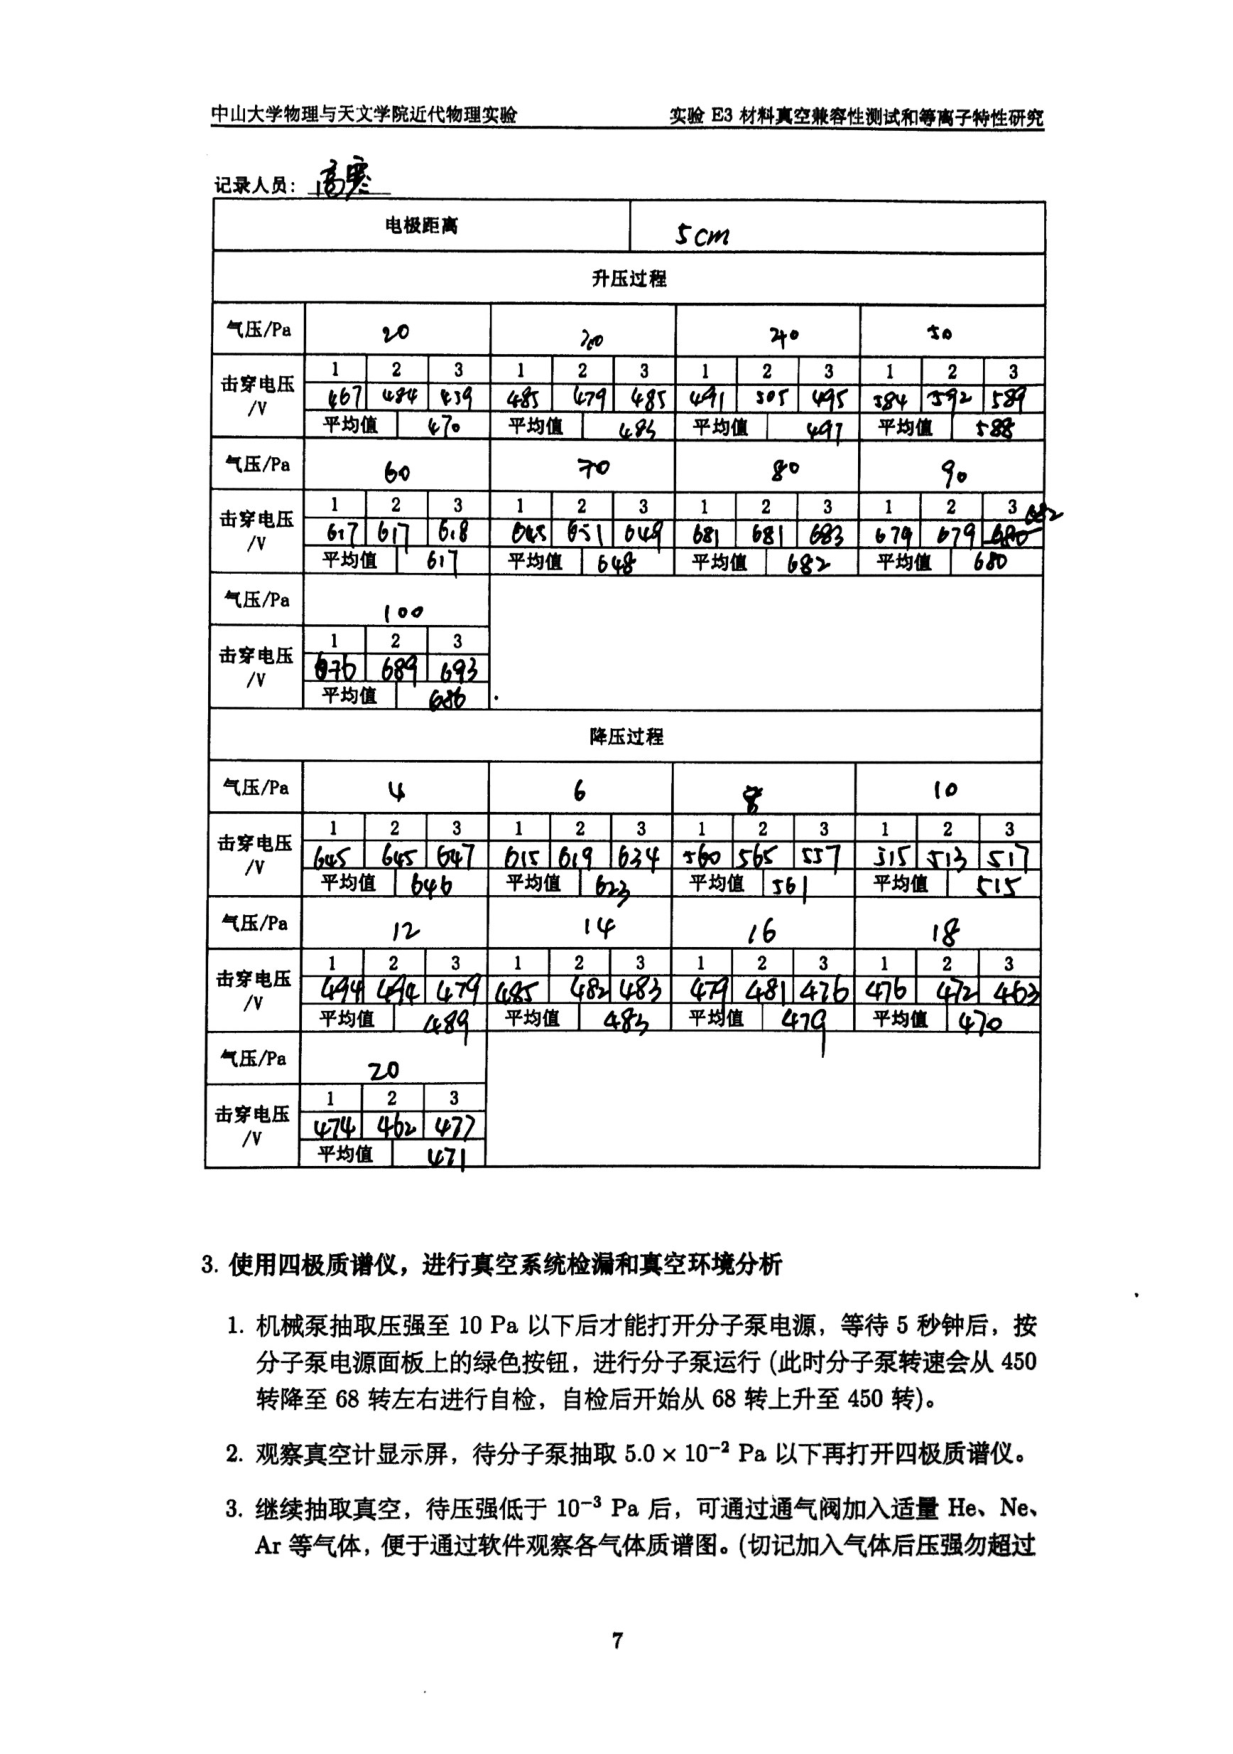
\includepdf[pages=1-3]{Record}

\newpage%分析与讨论
\cpic{0.255}{e3}%学生信息表格
\begin{center}
\LARGE\textbf{{\ExpeName}}
\end{center}
\textbf{【分析与讨论】}\\
1.\textbf{使用机械泵和分子泵获得高真空}\par
实验中，我们先利用机械泵获得了$\sim 10 \unit{Pa}$的真空，再利用分子泵获得了$\sim 10^{-5} \unit{Pa}$的高真空，整个过程约耗时半小时。
\emptyline
\\
2.\textbf{验证帕邢定律}\par
调整极板间距为$5\unit{cm}$，调节真空气压$V$，调节电压$p$使得剩余气体刚好被击穿，如\cref{sh1,sh2}。
\cpicn{0.09}{sh1}{剩余空气被高压击穿发出紫色辉光}
\cpicn{0.09}{sh2}{剩余空气被高压击穿发出紫色辉光}
测得$p-V$曲线如\cref{fit1}
\cpicn{0.4}{fit1}{极板间距为$5\unit{cm}$时的$p-V$曲线}
\par
重新调整极板间距为$4\unit{cm}$，调节真空气压$V$，调节电压$p$使得剩余气体刚好被击穿，测得$p-V$曲线如
\cpicn{0.4}{fit2}{极板间距为$4\unit{cm}$时的$p-V$曲线}
\par
为了得到更精确的结果，需要将帕邢定律的表达式线性化以进行拟合，得到各参数的值。首先有
\beq
V = \frac{BPd}{\ln{\frac{APd}{\ln(1+ 1/\gamma)}}}
\eeq
记
\bea
b&= Bd \\
a &= \frac{Ad}{\ln(1+ 1/\gamma)}
\eea
原公式写为
\beq
V = \frac{bP}{\ln aP}
\eeq
移项得到
\beq
\ln a + \ln P = \frac{bP}{V}
\eeq
或
\beq
\ln P = b \frac{P}{V} - \ln a
\eeq
因此以$\ln P$为纵坐标，$\frac{P}{V}$为横坐标，得到的结果理因是线性的。
\par
对
\emptyline
\\
3.\textbf{真空系统检漏和真空环境分析}\par
保持真空度为$\sim 1\times 10^{-2} \unit{Pa}$，改变分辨率和加速电压，得到几组扫描结果如\cref{1e-2_air_default,1e-2_air_resolu_30,96e-3_air_resolu_60_emi_01,96e-3_air_resolu_60_emi_02,96e-3_air_resolu_60_eVol_40,97e-3_air_resolu_20,97e-3_air_resolu_40,97e-3_air_resolu_50,98e-3_air_resolu_20,96e-3_air_resolu_60_eVol_80,96e-3_air_resolu_60}。
\cpicn{0.28}{1e-2_air_default}{真空度为$1\times 10^{-2} \unit{Pa}$默认设置下的扫描结果}
\cpicn{0.28}{1e-2_air_resolu_30}{真空度为$1\times 10^{-2} \unit{Pa}$改变分辨率为30下的扫描结果}
\cpicn{0.28}{96e-3_air_resolu_60_emi_01}{真空度为$0.96\times 10^{-2} \unit{Pa}$改变分辨率为60，发射系数为0.1下的扫描结果}
\cpicn{0.28}{96e-3_air_resolu_60_emi_02}{真空度为$0.96\times 10^{-2} \unit{Pa}$改变分辨率为60，发射系数为0.2下的扫描结果}
\cpicn{0.28}{96e-3_air_resolu_60_eVol_40}{真空度为$0.96\times 10^{-2} \unit{Pa}$改变分辨率为60，电压为40下的扫描结果}
\cpicn{0.28}{97e-3_air_resolu_20}{真空度为$0.97\times 10^{-2} \unit{Pa}$改变分辨率为20下的扫描结果}
\cpicn{0.28}{97e-3_air_resolu_40}{真空度为$0.97\times 10^{-2} \unit{Pa}$改变分辨率为40下的扫描结果}
\cpicn{0.28}{97e-3_air_resolu_50}{真空度为$0.97\times 10^{-2} \unit{Pa}$改变分辨率为50下的扫描结果}
\cpicn{0.28}{98e-3_air_resolu_20}{真空度为$0.98\times 10^{-2} \unit{Pa}$改变分辨率为20下的扫描结果}
\cpicn{0.28}{96e-3_air_resolu_60_eVol_80}{真空度为$0.97\times 10^{-2} \unit{Pa}$改变分辨率为60，电压为80下的扫描结果}
\cpicn{0.28}{96e-3_air_resolu_60}{真空度为$0.96\times 10^{-2} \unit{Pa}$改变分辨率为60下的扫描结果}
最强的吸收峰位于$28$处，由于
\beq
M_r(\ce{N2}) = A_r (\ce{N2}) + A_r (\ce{N2}) = 14\times 2 = 28
\eeq
峰对应\ce{N2+}离子，来源于剩余空气中的氮气；次强的吸收峰出现在$32$处，
由于
\beq
M_r(\ce{O2}) = A_r (\ce{O2}) + A_r (\ce{O2}) = 16\times 2 = 32
\eeq
峰对应\ce{O2+}离子，来源于剩余空气中的氧气。此外，位于$18$和$44$的吸收峰可能来源于水蒸气和\ce{CO2}的贡献
\beq
M_r (\ce{H2O}) = 2A_r (\ce{H}) + A_r(\ce{O}) = 2 + 16 = 18
\eeq
\beq
M_r(\ce{CO2}) = A_r(\ce{C}) + 2A_r(\ce{O}) = 12 + 2\times 16 = 44
\eeq
它们可能都来自于实验者的呼吸作用\cite{bio}
\beq
\ce{CH2OH(CHOH)_4CHO + 6H2O + 6O2 ->T[酶] 6CO2 + 12H2O}
\eeq
而位于$14$和$16$的峰可能来自\ce{N2^2+}和\ce{O2^2+}，他们是剩余空气的氮气和氧气二次电离产生的。\par
可以看到，改变各参数，曲线的尺度发生微小变化，但总的吸收峰不变。
\par
在真空腔内加入氦气至总压强为$8.4\times 10^{-3}\unit{Pa}$，得到的结果如\cref{84e-3_He_resolu_60_eVol_40_04,84e-3_He_resolu_60_eVol_40,84e-3_He_resolu_60_eVol_60,84e-3_He_resolu_60_eVol_80}
\cpicn{0.28}{84e-3_He_resolu_60_eVol_40_04}{真空度为$8.4\times 10^{-3}\unit{Pa}$改变分辨率为60下的扫描结果}
\cpicn{0.28}{84e-3_He_resolu_60_eVol_40}{真空度为$8.4\times 10^{-3}\unit{Pa}$改变分辨率为60，发射电压为40下的扫描结果}
\cpicn{0.28}{84e-3_He_resolu_60_eVol_60}{真空度为$8.4\times 10^{-3}\unit{Pa}$改变分辨率为60，发射电压为60下的扫描结果}
\cpicn{0.28}{84e-3_He_resolu_60_eVol_80}{真空度为$8.4\times 10^{-3}\unit{Pa}$改变分辨率为60，发射电压为80下的扫描结果}
吸收峰出现在4处，对应氦气。此外发现，改变发射电压，吸收峰几乎没有变化。
\par
在真空腔内加入氩气至总压强为$\sim 7 \times 10^{-3}\unit{Pa}$，得到的结果如\cref{68e-3_Ar_resolu_60_emi_02_eVol_40,69e-3_Ar_resolu_60_eVol_40,76e-3_Ar_resolu_60_eVol_60,77e-3_Ar_resolu_60_eVol_80}
\cpicn{0.28}{68e-3_Ar_resolu_60_emi_02_eVol_40}{真空度为$6.8\times 10^{-3}\unit{Pa}$改变发射系数为0.2，发射电压为40下的扫描结果}
\cpicn{0.28}{69e-3_Ar_resolu_60_eVol_40}{真空度为$6.9\times 10^{-3}\unit{Pa}$改变分辨率为60，发射电压为40下的扫描结果}
\cpicn{0.28}{76e-3_Ar_resolu_60_eVol_60}{真空度为$7.6\times 10^{-3}\unit{Pa}$改变分辨率为60，发射电压为60下的扫描结果}
\cpicn{0.28}{77e-3_Ar_resolu_60_eVol_80}{真空度为$7.7\times 10^{-3}\unit{Pa}$改变分辨率为60，发射电压为80下的扫描结果}
吸收峰出现在40处，对应氩气。此外发现，改变发射电压，吸收峰几乎没有变化。
\par
在真空腔内加入氩气至总压强为$\sim 7 \times 10^{-3}\unit{Pa}$，得到的结果如\cref{65e-3_Ne_resolu_60_eVol_40_02,65e-3_Ne_resolu_60_eVol_40_04,65e-3_Ne_resolu_60_eVol_60_02,65e-3_Ne_resolu_60_eVol_80_02}
\cpicn{0.28}{65e-3_Ne_resolu_60_eVol_40_02}{真空度为$6.8\times 10^{-3}\unit{Pa}$改变发射系数为0.2，发射电压为40下的扫描结果}
\cpicn{0.28}{65e-3_Ne_resolu_60_eVol_40_04}{真空度为$6.9\times 10^{-3}\unit{Pa}$改变发射系数为0.4，发射电压为40下的扫描结果}
\cpicn{0.28}{65e-3_Ne_resolu_60_eVol_60_02}{真空度为$7.6\times 10^{-3}\unit{Pa}$改变发射系数为0.2，发射电压为60下的扫描结果}
\cpicn{0.28}{65e-3_Ne_resolu_60_eVol_80_02}{真空度为$7.7\times 10^{-3}\unit{Pa}$改变发射系数为0.4，发射电压为80下的扫描结果}
吸收峰出现在20处，对应氩气。此外发现，改变发射电压，吸收峰几乎没有变化。
\emptyline
\\
\textbf{【实验思考题】}\par
见【实验前思考题】。

\bibliographystyle{IEEEtran}
\bibliography{model.bib}
\end{document}